% Tikz File 'mytikz.tex'
\documentclass{standalone}
\usepackage{amsmath,xparse}
\DeclareMathOperator{\vsd}{VSD}
\DeclareMathOperator{\asd}{ASD}
\DeclareMathOperator{\ea}{EA}
\DeclareMathOperator{\bb}{BB}
\DeclareMathOperator{\voc}{VC}
\usepackage{tikz}

\pgfdeclarelayer{bg} 
\pgfdeclarelayer{background}
\pgfdeclarelayer{foreground}
\pgfsetlayers{background,main,foreground}
\tikzstyle{sensor}=[draw, text width=2em, 
    text centered, minimum height=2.5em]
 \tikzstyle{v} =[circle, thick, minimum size=0.8cm, draw=black]

\begin{document}
 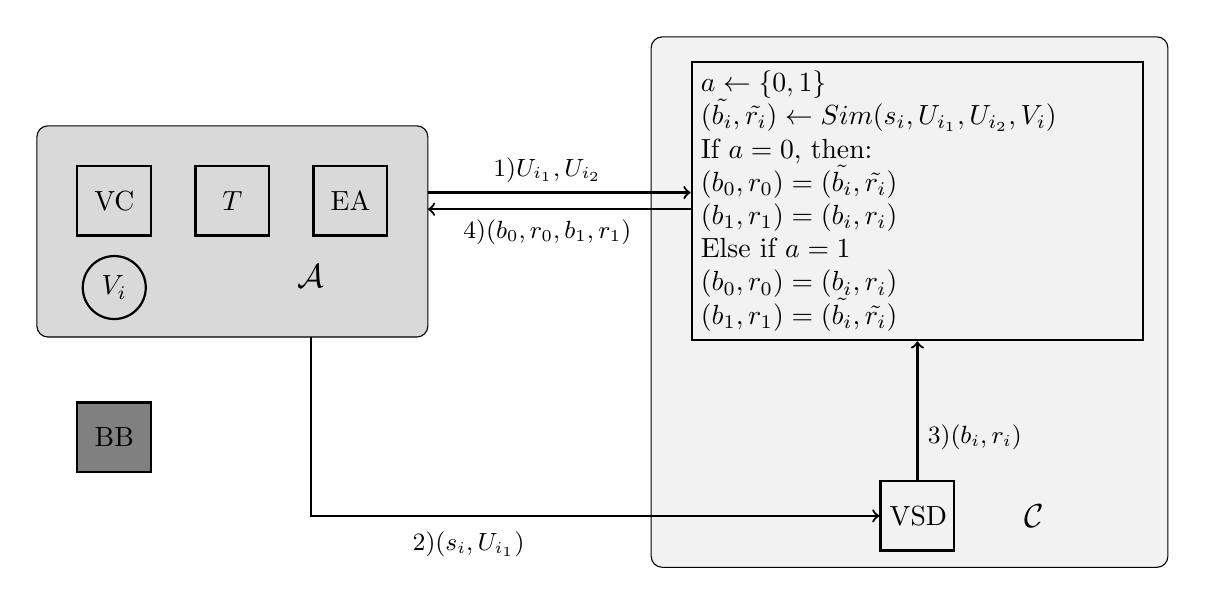
\begin{tikzpicture}[thick]
  \node[draw,rectangle]  at (-2, 5) (ea)[sensor] {$\ea$};
    \path (ea.south) +(-0.5,-0.5) node (a) {\large{$\mathcal{A}$}};
  \node[draw,rectangle,text width=5.5cm]  at (5.2, 5) (c) {$a \leftarrow \{0,1\} $ \\  $(\tilde{b_i}, \tilde{r_i}) \leftarrow Sim(s_i,U_{i_1},U_{i_2}, V_i)$\\If $a=0$, then:\\ $(b_0, r_0) = (\tilde{b_i},\tilde{r_i})$\\ $(b_1,r_1)= (b_i,r_i)$ \\ Else if $a = 1$ \\$(b_0,r_0) = (b_i,r_i) $ \\$(b_1, r_1) = (\tilde{b_i},\tilde{r_i})$};
   \node[draw,rectangle]  at (5.2, 1) (vsd)[sensor] { $\vsd$};
   \node[draw,rectangle]  at (-3.5, 5) (t)[sensor] { $T$};
      \node[draw,rectangle]  at (-5, 5) (vc)[sensor] { $\voc$};
         \node [ draw,circle] at (-5,3.9) (vfake)[v]{$V_i$};
      
           \node[draw,rectangle, fill = gray]  at (-5, 2) (bb)[sensor] { $\bb$};
   
   \draw[transform canvas={yshift=-0.7ex},->,shorten >=0.5cm] (c) node[font=\small, below,xshift=-4.7cm]  {$4) (b_0,r_0, b_1,r_1)$}  -- (ea);
      \draw[transform canvas={yshift=0.7ex},<-,shorten >=0.5cm] (c) node[font=\small, above,xshift=-4.7cm]  {$1) U_{i_1},U_{i_2}$}  -- (ea);
   
      \draw[->,shorten <=0.5cm] (a) node[font=\small, above,yshift=-3.7cm, xshift = 2cm] {$2) (s_i,U_{i_1})$} |- (vsd);
   
   \draw[<-] (c) node[font=\small, right,yshift=-3cm,] {$3) (b_i,r_i)$} -- (vsd);
   
     \begin{pgfonlayer}{background}
        \path (vc.west |- ea.north)+(-0.5,0.5) node (e) {};
        \path (a.south -| ea.east)+(+0.5,-0.5) node (d) {};
        \path[rounded corners, draw=black, fill = gray!30]
            (e) rectangle (d);
    \end{pgfonlayer} 
    
     \begin{pgfonlayer}{background}
        \path (c.west |- c.north)+(-0.5,0.3) node (a) {};
        \path (vsd.south -| c.east)+(+0.3,-0.2) node (b) {};
        \path[rounded corners, draw=black, fill = gray!10]
            (a) rectangle (b);
    \end{pgfonlayer}
    \path (vsd.east) +(+1,0) node (RE) {\large{$\mathcal{C}$}};
  \end{tikzpicture}
\end{document}